
%% bare_jrnl.tex
%% V1.3
%% 2007/01/11
%% by Michael Shell
%% see http://www.michaelshell.org/
%% for current contact information.
%%
%% This is a skeleton file demonstrating the use of IEEEtran.cls
%% (requires IEEEtran.cls version 1.7 or later) with an IEEE journal paper.
%%
%% Support sites:
%% http://www.michaelshell.org/tex/ieeetran/
%% http://www.ctan.org/tex-archive/macros/latex/contrib/IEEEtran/
%% and
%% http://www.ieee.org/



% *** Authors should verify (and, if needed, correct) their LaTeX system  ***
% *** with the testflow diagnostic prior to trusting their LaTeX platform ***
% *** with production work. IEEE's font choices can trigger bugs that do  ***
% *** not appear when using other class files.                            ***
% The testflow support page is at:
% http://www.michaelshell.org/tex/testflow/


%%*************************************************************************
%% Legal Notice:
%% This code is offered as-is without any warranty either expressed or
%% implied; without even the implied warranty of MERCHANTABILITY or
%% FITNESS FOR A PARTICULAR PURPOSE! 
%% User assumes all risk.
%% In no event shall IEEE or any contributor to this code be liable for
%% any damages or losses, including, but not limited to, incidental,
%% consequential, or any other damages, resulting from the use or misuse
%% of any information contained here.
%%
%% All comments are the opinions of their respective authors and are not
%% necessarily endorsed by the IEEE.
%%
%% This work is distributed under the LaTeX Project Public License (LPPL)
%% ( http://www.latex-project.org/ ) version 1.3, and may be freely used,
%% distributed and modified. A copy of the LPPL, version 1.3, is included
%% in the base LaTeX documentation of all distributions of LaTeX released
%% 2003/12/01 or later.
%% Retain all contribution notices and credits.
%% ** Modified files should be clearly indicated as such, including  **
%% ** renaming them and changing author support contact information. **
%%
%% File list of work: IEEEtran.cls, IEEEtran_HOWTO.pdf, bare_adv.tex,
%%                    bare_conf.tex, bare_jrnl.tex, bare_jrnl_compsoc.tex
%%*************************************************************************

% Note that the a4paper option is mainly intended so that authors in
% countries using A4 can easily print to A4 and see how their papers will
% look in print - the typesetting of the document will not typically be
% affected with changes in paper size (but the bottom and side margins will).
% Use the testflow package mentioned above to verify correct handling of
% both paper sizes by the user's LaTeX system.
%
% Also note that the "draftcls" or "draftclsnofoot", not "draft", option
% should be used if it is desired that the figures are to be displayed in
% draft mode.
%
\documentclass[journal]{IEEEtran}
%
% If IEEEtran.cls has not been installed into the LaTeX system files,
% manually specify the path to it like:
% \documentclass[journal]{../sty/IEEEtran}





% Some very useful LaTeX packages include:
% (uncomment the ones you want to load)


% *** MISC UTILITY PACKAGES ***
%
%\usepackage{ifpdf}
% Heiko Oberdiek's ifpdf.sty is very useful if you need conditional
% compilation based on whether the output is pdf or dvi.
% usage:
% \ifpdf
%   % pdf code
% \else
%   % dvi code
% \fi
% The latest version of ifpdf.sty can be obtained from:
% http://www.ctan.org/tex-archive/macros/latex/contrib/oberdiek/
% Also, note that IEEEtran.cls V1.7 and later provides a builtin
% \ifCLASSINFOpdf conditional that works the same way.
% When switching from latex to pdflatex and vice-versa, the compiler may
% have to be run twice to clear warning/error messages.






% *** CITATION PACKAGES ***
%
\usepackage{cite}
% cite.sty was written by Donald Arseneau
% V1.6 and later of IEEEtran pre-defines the format of the cite.sty package
% \cite{} output to follow that of IEEE. Loading the cite package will
% result in citation numbers being automatically sorted and properly
% "compressed/ranged". e.g., [1], [9], [2], [7], [5], [6] without using
% cite.sty will become [1], [2], [5]--[7], [9] using cite.sty. cite.sty's
% \cite will automatically add leading space, if needed. Use cite.sty's
% noadjust option (cite.sty V3.8 and later) if you want to turn this off.
% cite.sty is already installed on most LaTeX systems. Be sure and use
% version 4.0 (2003-05-27) and later if using hyperref.sty. cite.sty does
% not currently provide for hyperlinked citations.
% The latest version can be obtained at:
% http://www.ctan.org/tex-archive/macros/latex/contrib/cite/
% The documentation is contained in the cite.sty file itself.






% *** GRAPHICS RELATED PACKAGES ***
%
\ifCLASSINFOpdf
\usepackage[pdftex]{graphicx}
  % declare the path(s) where your graphic files are
  % \graphicspath{{../pdf/}{../jpeg/}}
  % and their extensions so you won't have to specify these with
  % every instance of \includegraphics
  % \DeclareGraphicsExtensions{.pdf,.jpeg,.png}
\else
  % or other class option (dvipsone, dvipdf, if not using dvips). graphicx
  % will default to the driver specified in the system graphics.cfg if no
  % driver is specified.
  % \usepackage[dvips]{graphicx}
  % declare the path(s) where your graphic files are
  % \graphicspath{{../eps/}}
  % and their extensions so you won't have to specify these with
  % every instance of \includegraphics
  % \DeclareGraphicsExtensions{.eps}
\fi
% graphicx was written by David Carlisle and Sebastian Rahtz. It is
% required if you want graphics, photos, etc. graphicx.sty is already
% installed on most LaTeX systems. The latest version and documentation can
% be obtained at: 
% http://www.ctan.org/tex-archive/macros/latex/required/graphics/
% Another good source of documentation is "Using Imported Graphics in
% LaTeX2e" by Keith Reckdahl which can be found as epslatex.ps or
% epslatex.pdf at: http://www.ctan.org/tex-archive/info/
%
% latex, and pdflatex in dvi mode, support graphics in encapsulated
% postscript (.eps) format. pdflatex in pdf mode supports graphics
% in .pdf, .jpeg, .png and .mps (metapost) formats. Users should ensure
% that all non-photo figures use a vector format (.eps, .pdf, .mps) and
% not a bitmapped formats (.jpeg, .png). IEEE frowns on bitmapped formats
% which can result in "jaggedy"/blurry rendering of lines and letters as
% well as large increases in file sizes.
%
% You can find documentation about the pdfTeX application at:
% http://www.tug.org/applications/pdftex


\usepackage{epstopdf}


% *** MATH PACKAGES ***
%
%\usepackage[cmex10]{amsmath}
% A popular package from the American Mathematical Society that provides
% many useful and powerful commands for dealing with mathematics. If using
% it, be sure to load this package with the cmex10 option to ensure that
% only type 1 fonts will utilized at all point sizes. Without this option,
% it is possible that some math symbols, particularly those within
% footnotes, will be rendered in bitmap form which will result in a
% document that can not be IEEE Xplore compliant!
%
% Also, note that the amsmath package sets \interdisplaylinepenalty to 10000
% thus preventing page breaks from occurring within multiline equations. Use:
%\interdisplaylinepenalty=2500
% after loading amsmath to restore such page breaks as IEEEtran.cls normally
% does. amsmath.sty is already installed on most LaTeX systems. The latest
% version and documentation can be obtained at:
% http://www.ctan.org/tex-archive/macros/latex/required/amslatex/math/





% *** SPECIALIZED LIST PACKAGES ***
%
%\usepackage{algorithmic}
% algorithmic.sty was written by Peter Williams and Rogerio Brito.
% This package provides an algorithmic environment fo describing algorithms.
% You can use the algorithmic environment in-text or within a figure
% environment to provide for a floating algorithm. Do NOT use the algorithm
% floating environment provided by algorithm.sty (by the same authors) or
% algorithm2e.sty (by Christophe Fiorio) as IEEE does not use dedicated
% algorithm float types and packages that provide these will not provide
% correct IEEE style captions. The latest version and documentation of
% algorithmic.sty can be obtained at:
% http://www.ctan.org/tex-archive/macros/latex/contrib/algorithms/
% There is also a support site at:
% http://algorithms.berlios.de/index.html
% Also of interest may be the (relatively newer and more customizable)
% algorithmicx.sty package by Szasz Janos:
% http://www.ctan.org/tex-archive/macros/latex/contrib/algorithmicx/




% *** ALIGNMENT PACKAGES ***
%
%\usepackage{array}
% Frank Mittelbach's and David Carlisle's array.sty patches and improves
% the standard LaTeX2e array and tabular environments to provide better
% appearance and additional user controls. As the default LaTeX2e table
% generation code is lacking to the point of almost being broken with
% respect to the quality of the end results, all users are strongly
% advised to use an enhanced (at the very least that provided by array.sty)
% set of table tools. array.sty is already installed on most systems. The
% latest version and documentation can be obtained at:
% http://www.ctan.org/tex-archive/macros/latex/required/tools/


%\usepackage{mdwmath}
%\usepackage{mdwtab}
% Also highly recommended is Mark Wooding's extremely powerful MDW tools,
% especially mdwmath.sty and mdwtab.sty which are used to format equations
% and tables, respectively. The MDWtools set is already installed on most
% LaTeX systems. The lastest version and documentation is available at:
% http://www.ctan.org/tex-archive/macros/latex/contrib/mdwtools/


% IEEEtran contains the IEEEeqnarray family of commands that can be used to
% generate multiline equations as well as matrices, tables, etc., of high
% quality.


%\usepackage{eqparbox}
% Also of notable interest is Scott Pakin's eqparbox package for creating
% (automatically sized) equal width boxes - aka "natural width parboxes".
% Available at:
% http://www.ctan.org/tex-archive/macros/latex/contrib/eqparbox/





% *** SUBFIGURE PACKAGES ***
\usepackage[tight,footnotesize]{subfigure}
% subfigure.sty was written by Steven Douglas Cochran. This package makes it
% easy to put subfigures in your figures. e.g., "Figure 1a and 1b". For IEEE
% work, it is a good idea to load it with the tight package option to reduce
% the amount of white space around the subfigures. subfigure.sty is already
% installed on most LaTeX systems. The latest version and documentation can
% be obtained at:
% http://www.ctan.org/tex-archive/obsolete/macros/latex/contrib/subfigure/
% subfigure.sty has been superceeded by subfig.sty.



%\usepackage[caption=false]{caption}
%\usepackage[font=footnotesize]{subfig}
% subfig.sty, also written by Steven Douglas Cochran, is the modern
% replacement for subfigure.sty. However, subfig.sty requires and
% automatically loads Axel Sommerfeldt's caption.sty which will override
% IEEEtran.cls handling of captions and this will result in nonIEEE style
% figure/table captions. To prevent this problem, be sure and preload
% caption.sty with its "caption=false" package option. This is will preserve
% IEEEtran.cls handing of captions. Version 1.3 (2005/06/28) and later 
% (recommended due to many improvements over 1.2) of subfig.sty supports
% the caption=false option directly:
%\usepackage[caption=false,font=footnotesize]{subfig}
%
% The latest version and documentation can be obtained at:
% http://www.ctan.org/tex-archive/macros/latex/contrib/subfig/
% The latest version and documentation of caption.sty can be obtained at:
% http://www.ctan.org/tex-archive/macros/latex/contrib/caption/




% *** FLOAT PACKAGES ***
%
%\usepackage{fixltx2e}
% fixltx2e, the successor to the earlier fix2col.sty, was written by
% Frank Mittelbach and David Carlisle. This package corrects a few problems
% in the LaTeX2e kernel, the most notable of which is that in current
% LaTeX2e releases, the ordering of single and double column floats is not
% guaranteed to be preserved. Thus, an unpatched LaTeX2e can allow a
% single column figure to be placed prior to an earlier double column
% figure. The latest version and documentation can be found at:
% http://www.ctan.org/tex-archive/macros/latex/base/



%\usepackage{stfloats}
% stfloats.sty was written by Sigitas Tolusis. This package gives LaTeX2e
% the ability to do double column floats at the bottom of the page as well
% as the top. (e.g., "\begin{figure*}[!b]" is not normally possible in
% LaTeX2e). It also provides a command:
%\fnbelowfloat
% to enable the placement of footnotes below bottom floats (the standard
% LaTeX2e kernel puts them above bottom floats). This is an invasive package
% which rewrites many portions of the LaTeX2e float routines. It may not work
% with other packages that modify the LaTeX2e float routines. The latest
% version and documentation can be obtained at:
% http://www.ctan.org/tex-archive/macros/latex/contrib/sttools/
% Documentation is contained in the stfloats.sty comments as well as in the
% presfull.pdf file. Do not use the stfloats baselinefloat ability as IEEE
% does not allow \baselineskip to stretch. Authors submitting work to the
% IEEE should note that IEEE rarely uses double column equations and
% that authors should try to avoid such use. Do not be tempted to use the
% cuted.sty or midfloat.sty packages (also by Sigitas Tolusis) as IEEE does
% not format its papers in such ways.


%\ifCLASSOPTIONcaptionsoff
%  \usepackage[nomarkers]{endfloat}
% \let\MYoriglatexcaption\caption
% \renewcommand{\caption}[2][\relax]{\MYoriglatexcaption[#2]{#2}}
%\fi
% endfloat.sty was written by James Darrell McCauley and Jeff Goldberg.
% This package may be useful when used in conjunction with IEEEtran.cls'
% captionsoff option. Some IEEE journals/societies require that submissions
% have lists of figures/tables at the end of the paper and that
% figures/tables without any captions are placed on a page by themselves at
% the end of the document. If needed, the draftcls IEEEtran class option or
% \CLASSINPUTbaselinestretch interface can be used to increase the line
% spacing as well. Be sure and use the nomarkers option of endfloat to
% prevent endfloat from "marking" where the figures would have been placed
% in the text. The two hack lines of code above are a slight modification of
% that suggested by in the endfloat docs (section 8.3.1) to ensure that
% the full captions always appear in the list of figures/tables - even if
% the user used the short optional argument of \caption[]{}.
% IEEE papers do not typically make use of \caption[]'s optional argument,
% so this should not be an issue. A similar trick can be used to disable
% captions of packages such as subfig.sty that lack options to turn off
% the subcaptions:
% For subfig.sty:
% \let\MYorigsubfloat\subfloat
% \renewcommand{\subfloat}[2][\relax]{\MYorigsubfloat[]{#2}}
% For subfigure.sty:
% \let\MYorigsubfigure\subfigure
% \renewcommand{\subfigure}[2][\relax]{\MYorigsubfigure[]{#2}}
% However, the above trick will not work if both optional arguments of
% the \subfloat/subfig command are used. Furthermore, there needs to be a
% description of each subfigure *somewhere* and endfloat does not add
% subfigure captions to its list of figures. Thus, the best approach is to
% avoid the use of subfigure captions (many IEEE journals avoid them anyway)
% and instead reference/explain all the subfigures within the main caption.
% The latest version of endfloat.sty and its documentation can obtained at:
% http://www.ctan.org/tex-archive/macros/latex/contrib/endfloat/
%
% The IEEEtran \ifCLASSOPTIONcaptionsoff conditional can also be used
% later in the document, say, to conditionally put the References on a 
% page by themselves.





% *** PDF, URL AND HYPERLINK PACKAGES ***
%
\usepackage{url}
% url.sty was written by Donald Arseneau. It provides better support for
% handling and breaking URLs. url.sty is already installed on most LaTeX
% systems. The latest version can be obtained at:
% http://www.ctan.org/tex-archive/macros/latex/contrib/misc/
% Read the url.sty source comments for usage information. Basically,
% \url{my_url_here}.





% *** Do not adjust lengths that control margins, column widths, etc. ***
% *** Do not use packages that alter fonts (such as pslatex).         ***
% There should be no need to do such things with IEEEtran.cls V1.6 and later.
% (Unless specifically asked to do so by the journal or conference you plan
% to submit to, of course. )


% correct bad hyphenation here
\hyphenation{op-tical net-works semi-conduc-tor}


\begin{document}
%
% paper title
% can use linebreaks \\ within to get better formatting as desired
\title{Real-Time Implementation of Synchrophasor-based Wide-Area Power Oscillation Damping Control System}
%
%
% author names and IEEE memberships
% note positions of commas and nonbreaking spaces ( ~ ) LaTeX will not break
% a structure at a ~ so this keeps an author's name from being broken across
% two lines.
% use \thanks{} to gain access to the first footnote area
% a separate \thanks must be used for each paragraph as LaTeX2e's \thanks
% was not built to handle multiple paragraphs
%

%%Fix Later : Move Luigi as first author.

\author{Luigi~Vanfretti, Eldrich~Rebello,~\IEEEmembership{Non-Member,~IEEE,}
        Muhammad~Shoaib~Almas,~\IEEEmembership{Fellow,~OSA,}
        and~Luigi~Vanfretti,~\IEEEmembership{Senior~Member,~IEEE}% <-this % stops a space
\thanks{Eldrich Rebello has completed his Master's degree the School of Electrical Engineering, Aalto University, Helsinki, Finland
e-mail: eldrich.rebello@aalto.fi}% <-this % stops a space
\thanks{M. Shoaib Almas and L. Vanfretti are with KTH Royal Institute of Technology, Stockholm, Sweden. Email: msalmas@kth.se luigiv@kth.se}% <-this % stops a space
\thanks{This project was supported in part by the Nordic
Energy Research through the STRON$g^{2}$rid project.}}

% note the % following the last \IEEEmembership and also \thanks - 
% these prevent an unwanted space from occurring between the last author name
% and the end of the author line. i.e., if you had this:
% 
% \author{....lastname \thanks{...} \thanks{...} }
%                     ^------------^------------^----Do not want these spaces!
%
% a space would be appended to the last name and could cause every name on that
% line to be shifted left slightly. This is one of those "LaTeX things". For
% instance, "\textbf{A} \textbf{B}" will typeset as "A B" not "AB". To get
% "AB" then you have to do: "\textbf{A}\textbf{B}"
% \thanks is no different in this regard, so shield the last } of each \thanks
% that ends a line with a % and do not let a space in before the next \thanks.
% Spaces after \IEEEmembership other than the last one are OK (and needed) as
% you are supposed to have spaces between the names. For what it is worth,
% this is a minor point as most people would not even notice if the said evil
% space somehow managed to creep in.



% The paper headers
\markboth{Journal of \LaTeX\ Class Files,~Vol.~6, No.~1, August~2014}%
{Shell \MakeLowercase{\textit{et al.}}: Bare Demo of IEEEtran.cls for Journals}
% The only time the second header will appear is for the odd numbered pages
% after the title page when using the twoside option.
% 
% *** Note that you probably will NOT want to include the author's ***
% *** name in the headers of peer review papers.                   ***
% You can use \ifCLASSOPTIONpeerreview for conditional compilation here if
% you desire.




% If you want to put a publisher's ID mark on the page you can do it like
% this:
%\IEEEpubid{0000--0000/00\$00.00~\copyright~2007 IEEE}
% Remember, if you use this you must call \IEEEpubidadjcol in the second
% column for its text to clear the IEEEpubid mark.



% use for special paper notices
%\IEEEspecialpapernotice{(Invited Paper)}




% make the title area
\maketitle


\begin{abstract}
%\boldmath
The modern power grid is increasingly being used under operating conditions of increasing stress for which it was not designed. The increasing penetration levels of variable energy sources such as wind present significant grid stability issues. One of these stability issues is the phenomenon of low frequency, electro-mechanically induced, inter-area oscillations. Simulations have demonstrated the potential of Wide Area Measurement Signals (WAMS)-based Power Oscillation Damping (POD) in achieving improved electromechanical mode damping compared to traditional, local signal based, Power System Stabilizers (PSS). \iffalse Also, the adoption of synchrophasor measurement data from Phasor Measurement Units (PMU's) is rising annually.\fi This paper takes an established Phasor-based oscillation damping algorithm and combines it with modern PMU technology to implement a hardware prototype of a real-time oscillation damping control system using remote PMU signals sent over a communications network. The developed prototype is tested in real-time using a Hardware-in-the-loop approach in conjunction with the Klein-Rogers-Kundur two-area four-machine test system and is demonstrated to have applications independent of the controlled device.

%The developed hardware prototype has been tested using Real-Time hardware-in-the-loop (HIL) approach and the simulations are performed on Klien-Roger-Kundur two area four machine test system. 

\end{abstract}
% IEEEtran.cls defaults to using nonbold math in the Abstract.
% This preserves the distinction between vectors and scalars. However,
% if the journal you are submitting to favors bold math in the abstract,
% then you can use LaTeX's standard command \boldmath at the very start
% of the abstract to achieve this. Many IEEE journals frown on math
% in the abstract anyway.

% Note that keywords are not normally used for peerreview papers.
\begin{IEEEkeywords}
WAPOD, WAMPAC, synchrophasor, PMU, damping control, Wide Area measurement and control
\end{IEEEkeywords}






% For peer review papers, you can put extra information on the cover
% page as needed:
% \ifCLASSOPTIONpeerreview
% \begin{center} \bfseries EDICS Category: 3-BBND \end{center}
% \fi
%
% For peerreview papers, this IEEEtran command inserts a page break and
% creates the second title. It will be ignored for other modes.
\IEEEpeerreviewmaketitle



\section{Introduction}
% The very first letter is a 2 line initial drop letter followed
% by the rest of the first word in caps.
% 
% form to use if the first word consists of a single letter:
% \IEEEPARstart{A}{demo} file is ....
% 
% form to use if you need the single drop letter followed by
% normal text (unknown if ever used by IEEE):
% \IEEEPARstart{A}{}demo file is ....
% 
% Some journals put the first two words in caps:
% \IEEEPARstart{T}{his demo} file is ....
% 
% Here we have the typical use of a "T" for an initial drop letter
% and "HIS" in caps to complete the first word.
\IEEEPARstart{T}{he} goal of this paper is to demonstrate both the potential and flexibility in oscillation damping controller design that is possible by using synchrophasors (C37.118). The Phasor Power Oscillation Damping (Phasor POD) algorithm originally developed by \"{A}ngquist and Gama\cite{PhasorPOD} is run on a National Instruments Compact Reconfigurable Input / Output (cRIO) real-time controller. A slightly modified, \textsc{Simulink} model of the four-machine, two-area network developed by Klein-Rogers and Kundur \cite{KundurTwoArea} is run on the eMEGASIM \cite{eMEGASIM} platform from OPAL RT. This allows interfacing an externally generated control signal with the simulated model in real-time. This HIL\footnote{Hardware-in-the-loop} test is set up to verify the performance of the hardware implementation of the Phasor POD algorithm. The flexibility of the developed controller is also demonstrated by extracting various data from the synchrophasor input and using each as a damping input to the controller. That the controller can have multiple applications is demonstrated by testing it with two different controlled devices; a generator AVR system and a FACTS-device excitation system. A brief analysis of the performance of each input is also presented.\\

This paper is organised as follows:\\

Section \ref{Background} presents a brief background of the work together with the hardware and software architectures implemented. An outline of the two-area model, the hardware used and finally, an outline of the whole HIL test setup is also presented.\\

Section \ref{SetupPreparation} covers the preparation of the \textsc{Simulink} models for real-time simulation and the modifications made for this. Two test cases are examined, one with the WAPOD input fed to the excitation system of an SVC and the other with the WAPOD modulating the input of a generator AVR.\\

The results obtained from the two tests are presented and examined in Section \ref{Results}.\\

Section \ref{Challenges} outlines some of the major challenges and problems faced in the development, implementation and testing of this WAPOD controller including software challenges and the difficulties faced when dealing with real-world, analogue signals compared to pure simulations.\\

No experimental implementation is ever field-ready and there is always room for tremendous improvement. This is outlined in Section \ref{Future} and finally conclusions are drawn in Section \ref{Conclusion}.




% You must have at least 2 lines in the paragraph with the drop letter
% (should never be an issue)

%\hfill mds
 
%\hfill January 11, 2007

\section{Background}\label{Background}
As modern power systems grow in size, both in terms of power transfer capacity and geographic spread, they are increasingly being used for purposes that the power system was not designed for. Examples of these \textquoteleft new\textquoteright ~uses include conditions of increasing stress such as power trading between countries. These interconnections, which link synchronous generators, often separated by vast physical distances, create conditions where small disturbances can excite oscillations that may or may not settle. When the generators of one area oscillate at a low frequency (typically 0.2\textendash 2.5Hz) against the generators of another interconnected, but distinct area, \textquoteleft inter-area\textquoteright ~oscillations may start.\\

Although the purpose of system interconnection was to increase stability, the present situation of the power system incorporates renewable energy sources and power trading corridors, both of which impact system stability. More modern solutions to the problems of inter area and intra oscillations use Power System Stabilizers (PSS) \cite{Dmello}. While a PSS provides excellent damping to intra area modes with good local observability, its performance with intra-area modes may not be satisfactory \cite{localREMcomparison}.\\

% needed in second column of first page if using \IEEEpubid
%\IEEEpubidadjcol

\subsection{Previous Experiences}

One important reason for choosing the Phasor-POD algorithm for real-time implementation was the fact that the algorithm uses few inputs and is independent of network configuration and topology. The only algorithm parameter that is network-dependent is the oscillation frequency and this is usually known from system studies. Compared to conventional, linearisation-based controllers, the adoption of phasor-based controllers has not been high mainly due to the fact that such controllers tend to be highly non-linear and thus difficult to model in simulation studies \cite{Chaudhuri}.

\subsection{Hardware Architecture}

The Wide Area Power Oscillation Damper (WAPOD)\footnote{Historically, damping stabilizers have been termed WAPOD where the P represents a measurement of active power through the line. Active power here would be used as a controller input signal. Although this term is not accurate when other quantities are used as control inputs or feedback signals, the term is used here to maintain consistency with existing literature.} prototype developed here uses commercially available micro-controller hardware and is based entirely on PMU measurements received over a TCP/IP network. The Phasor-POD algorithm \cite{PhasorPOD} will be implemented on a general purpose micro-controller and will be run in real-time. The inputs to the controller will come from one or multiple PMU's, each monitoring data at different points in the power system. The power system model used in this paper is the two-area four-machine model, originally proposed by Klein, Rogers and Kundur \cite{KundurTwoArea}. To prove the real-world applicability of the developed controller, all tests are carried out in real-time, with conditions such as noise and network transport delay present.\\

All real-time simulations here are performed on OPAL RT's e\textsc{Megasim} \cite{OPALemegasim} real-time simulation platform. \textsc{Simulink} models are executed in real-time and are interfaced with externally generated signals. Current and voltage signals from different points on the simulated network are extracted, amplified and then supplied as the input to two PMU's. Two cRIO-9076 \cite{cRIO9076} devices are used as PMU's. The synchrophasor data stream from these devices is streamed over a TCP/IP network to a Phasor Data Concentrator which produces a time-aligned output stream. This stream is then accessed, via a TCP/IP network, on a PC running LabVIEW which extracts raw measurement data. This extracted data is streamed over the network to a cRIO-9081 which runs the Phasors-POD algorithm in real-time. The FPGA on the cRIO-9081 \cite{cRIO9081} generates a damping signal which is then wired to the real-time simulator for use in the \textsc{Simulink} model.\\

\begin{figure}[!h]
\centering
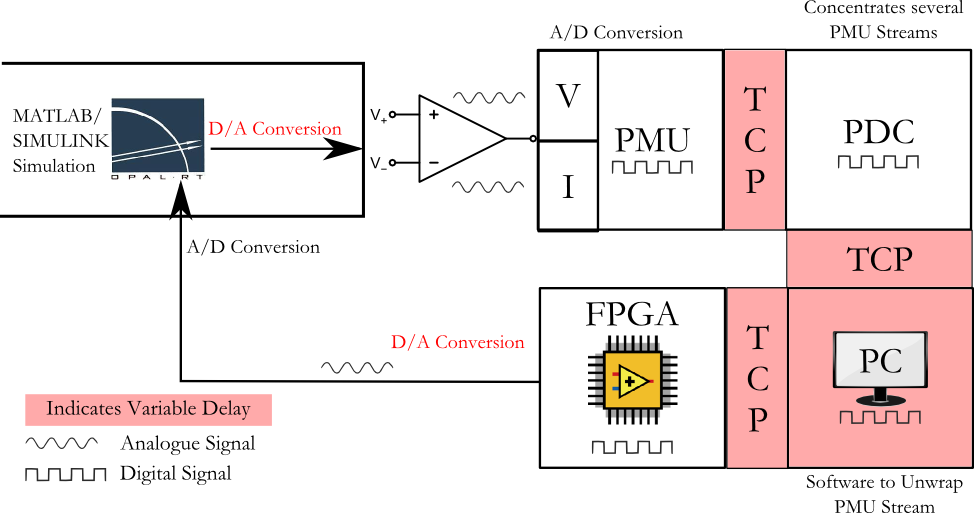
\includegraphics[width=3.5in]{DataFlow.png} 
\caption{Harware Outline showing complete data path}
\label{Hardware_Outline}
\end{figure}

Vanfretti et. al. describe the details of the equipment used here in \cite{SmarTSLab}. An image of the physical setup is included for clarity in Appendix \ref{SetupImage}. It is important to note that the data flow in Figure~\ref{Hardware_Outline} involves both D/A and A/D conversions. Also, since no synchronisation is used for these conversions, it is important that the sample rates or loop rates of each section be integer multiples of each other. This will prevent data value errors. The issue of different loop rates is covered in Section \ref{looprate}.\\

\subsection{Software Architecture}
The two-area four-machine model used here is available in \textsc{Simulink}'s SimPowerSystems and can be accessed by typing \texttt{power\_PSS} as a \textsc{Matlab} command. The \textsc{Simulink} implementation of the Phasor-POD algorithm was developed by Almas and Vanfretti \cite{PhasorPODImplement}. The Phasor-POD algorithm essentially separates an input signal into an average valued and an oscillating component. The oscillating component when suitably phase-shifted can be used as a supplementary damping input to a generator's AVR or the excitation system of a FACTS device.\\

LabVIEW's Real Time and FPGA modules were used to write the code for the respective sections of the cRIO. Also,  since no synchrophasor data-extraction software was capable of running independently on the RT controller, the process of extracting raw measurement data from the synchrophasor data stream was performed on a desktop computer. The software used for this was identical to that in \cite{SDK} and would run on a workstation computer, extract data from the PMU stream and send this extracted data to a LabVIEW program running on the same computer \cite{SDK}. \\

\subsection{Real-Time Implementation of Phasor-POD Algorithm}

The hardware implementation of the POD was based on the Compact Reconfigurable Input / Output (cRIO) 9081 \cite{cRIO9081} from National Instruments. This controller is equipped with an on-board Field Programmable Gate Array (FPGA) running at 400MHz in addition to an independent real-time controller. The real-time implementation of the Phasor-POD algorithm was based on the \textsc{Simulink} implementation by Almas \& Vanfretti \cite{PhasorPODImplement} and its goal was the replicate the behaviour of the \textsc{Simulink} implementation as closely as possible. The algorithm accepts three inputs; the search frequency, $\omega_{cs1}$, the sampling time $T_{s}$, the phase correction $alpha$ and a signal scaling factor. It takes advantage of the fact that the oscillation frequency for a given network configuration is usually known, which in this case is the 0.64Hz inter-area mode. Using this known frequency value, a  co-ordinate system, rotating at this known frequency, is set up where the oscillating component is continuously extracted as a phasor \cite{PhasorPOD}.\\
%update figure to show that Local control function was NOT implemented. Future work!-----------------------------------------------------------------------------
\begin{figure}[!t]
\centering
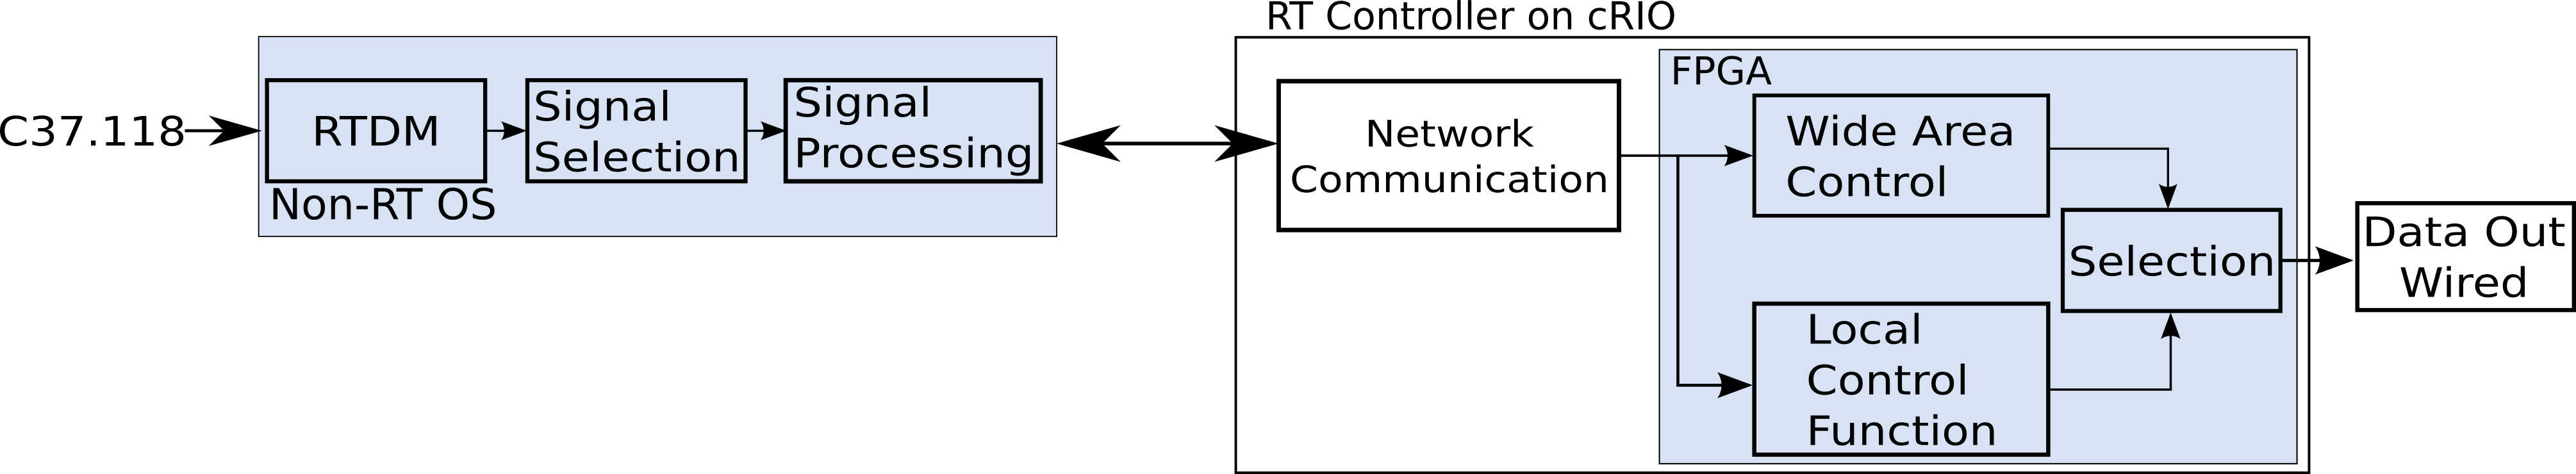
\includegraphics[width=3.5in]{Final_RT_Arch.png} 
\caption{RT Controller Architecture. The local control function is not implemented in this work} %showing future expandability with Local control function
\label{RTArchitecture}
\end{figure}

A three-layer, modular code architecture, based on an available template \cite{LabviewTemplate} was selected for implementation. An outline of the architecture is shown in Figure \ref{RTArchitecture} and each of the three layers are outlined below. 

\begin{itemize}
\item Core FPGA Software : Interacts with hardware terminals for I/O and runs Phasor-POD algorithm

\item Real Time (RT) Software : Manages network communication to remote terminal and also generates performance monitoring data

\item Remote Interface: Runs on workstation computer: Used to update algorithm parameters and monitor data \& performance. This layer is non deterministic.
\end{itemize}

The Phasor-POD algorithm could be implemented on either the real-time section of the cRIO or the FPGA but was implemented on the FPGA. This decision was made keeping in mind the computational resources and response speed needed to match the step size of the real-time simulator. The complexity of the code meant that the cRIO\rq{s} real-time controller would not be able to complete an iteration of the algorithm in the required 50$\mu$s response time. The real-time section of the cRIO handles network communication. Its primary purpose is to receive measurement data that the workstation computer extracts and to stream this data to the Phasor-POD algorithm running on the FPGA. The real-time controller also handles commands coming from the user interface running on the workstation computer.  It also monitors the output of the FPGA, sends data to the user interface for monitoring, periodically logs input and output data and handles error  conditions.\\

The remote interface runs in LabVIEW on a conventional Windows\textregistered~based computer. The Phasor-POD algorithm can be controlled from this interface. Also, the algorithm parameters can be set and modified. Since the operating system here is not real-time but is multi-tasking, the execution speed depends on the processor load and is not deterministic. Statnett's Synchrophasor Software Development Kit ($S^{3}DK$) was used to unwrap the PMU streams coming from the PDC and extract phasor measurements \cite{SDK}. This allowed for data to be extracted and used directly in the LabVIEW environment. Since the PMU reporting rate was 50 messages a second, new data was available every 20ms. The loop rate used by the $S^{3}DK$ was hence 20ms. The selection of a input for the controller and the computations required are performed here. For example, if active power is to be used as a POD input, voltage and current values must be multiplied to obtain the active power. If the voltage angle difference is to be used as an input, the required calculations are performed in this VI.\\

%This format for equations does not work. Why?---------------------------------

%\begin{equation} \label{phasoreqn}
%\left(t\right)={s}_{avg}+\mathrm{Re}\left\{{\stackrel{\to }{s}}_{ph}\cdot %{e}^{{j}^{wt}}\right\} \cite{Chaudhuri}
%\end{equation} 

%Include equation if needed---------------------------------

%$\left(t\right)={s}_{avg}+\mathrm{Re}\left\{{\stackrel{\to }{s}}_{ph}\cdot %{e}^{{j}^{wt}}\right\}$ \cite{Chaudhuri}

% An example of a floating figure using the graphicx package.
% Note that \label must occur AFTER (or within) \caption.
% For figures, \caption should occur after the \includegraphics.
% Note that IEEEtran v1.7 and later has special internal code that
% is designed to preserve the operation of \label within \caption
% even when the captionsoff option is in effect. However, because
% of issues like this, it may be the safest practice to put all your
% \label just after \caption rather than within \caption{}.
%
% Reminder: the "draftcls" or "draftclsnofoot", not "draft", class
% option should be used if it is desired that the figures are to be
% displayed while in draft mode.
%
%\begin{figure}[!t]
%\centering
%\includegraphics[width=2.5in]{myfigure}
% where an .eps filename suffix will be assumed under latex, 
% and a .pdf suffix will be assumed for pdflatex; or what has been declared
% via \DeclareGraphicsExtensions.
%\caption{Simulation Results}
%\label{fig_sim}
%\end{figure}

% Note that IEEE typically puts floats only at the top, even when this
% results in a large percentage of a column being occupied by floats.


% An example of a double column floating figure using two subfigures.
% (The subfig.sty package must be loaded for this to work.)
% The subfigure \label commands are set within each subfloat command, the
% \label for the overall figure must come after \caption.
% \hfil must be used as a separator to get equal spacing.
% The subfigure.sty package works much the same way, except \subfigure is
% used instead of \subfloat.
%
%\begin{figure*}[!t]
%\centerline{\subfloat[Case I]\includegraphics[width=2.5in]{subfigcase1}%
%\label{fig_first_case}}
%\hfil
%\subfloat[Case II]{\includegraphics[width=2.5in]{subfigcase2}%
%\label{fig_second_case}}}
%\caption{Simulation results}
%\label{fig_sim}
%\end{figure*}
%
% Note that often IEEE papers with subfigures do not employ subfigure
% captions (using the optional argument to \subfloat), but instead will
% reference/describe all of them (a), (b), etc., within the main caption.


% An example of a floating table. Note that, for IEEE style tables, the 
% \caption command should come BEFORE the table. Table text will default to
% \footnotesize as IEEE normally uses this smaller font for tables.
% The \label must come after \caption as always.
%
%\begin{table}[!t]
%% increase table row spacing, adjust to taste
%\renewcommand{\arraystretch}{1.3}
% if using array.sty, it might be a good idea to tweak the value of
% \extrarowheight as needed to properly center the text within the cells
%\caption{An Example of a Table}
%\label{table_example}
%\centering
%% Some packages, such as MDW tools, offer better commands for making tables
%% than the plain LaTeX2e tabular which is used here.
%\begin{tabular}{|c||c|}
%\hline
%One & Two\\
%\hline
%Three & Four\\
%\hline
%\end{tabular}
%\end{table}


% Note that IEEE does not put floats in the very first column - or typically
% anywhere on the first page for that matter. Also, in-text middle ("here")
% positioning is not used. Most IEEE journals use top floats exclusively.
% Note that, LaTeX2e, unlike IEEE journals, places footnotes above bottom
% floats. This can be corrected via the \fnbelowfloat command of the
% stfloats package.

\section{Setup Preparation}\label{SetupPreparation}

The nature of the Phasor-POD algorithm is generic enough to allow it to be used as a modulating input to a variety of controlled devices. Two examples are illustrated in this work, one, as a generator AVR modulating input and the other as a modulating input to the excitation system of a FACTS device (here, an SVC\footnote{Static VAR Compensator}). Figure \ref{NetworkOutline} illustrates both these uses along with the two-area network outline. Note that both possibilities are not implemented simultaneously.

\subsection{Two-Area Model Preparation - Generator AVR}

\begin{figure}[!th]
\centering
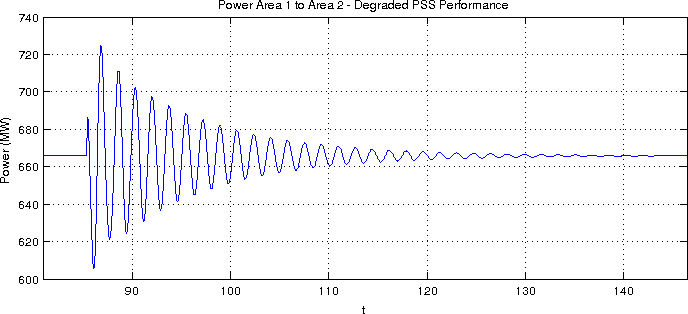
\includegraphics[width=3.5in]{PSS_degraded_performance.png}
\caption{Degraded performance with PSS}
\label{PSS_Degrade}
\end{figure}

\begin{figure}[!th]
\centering
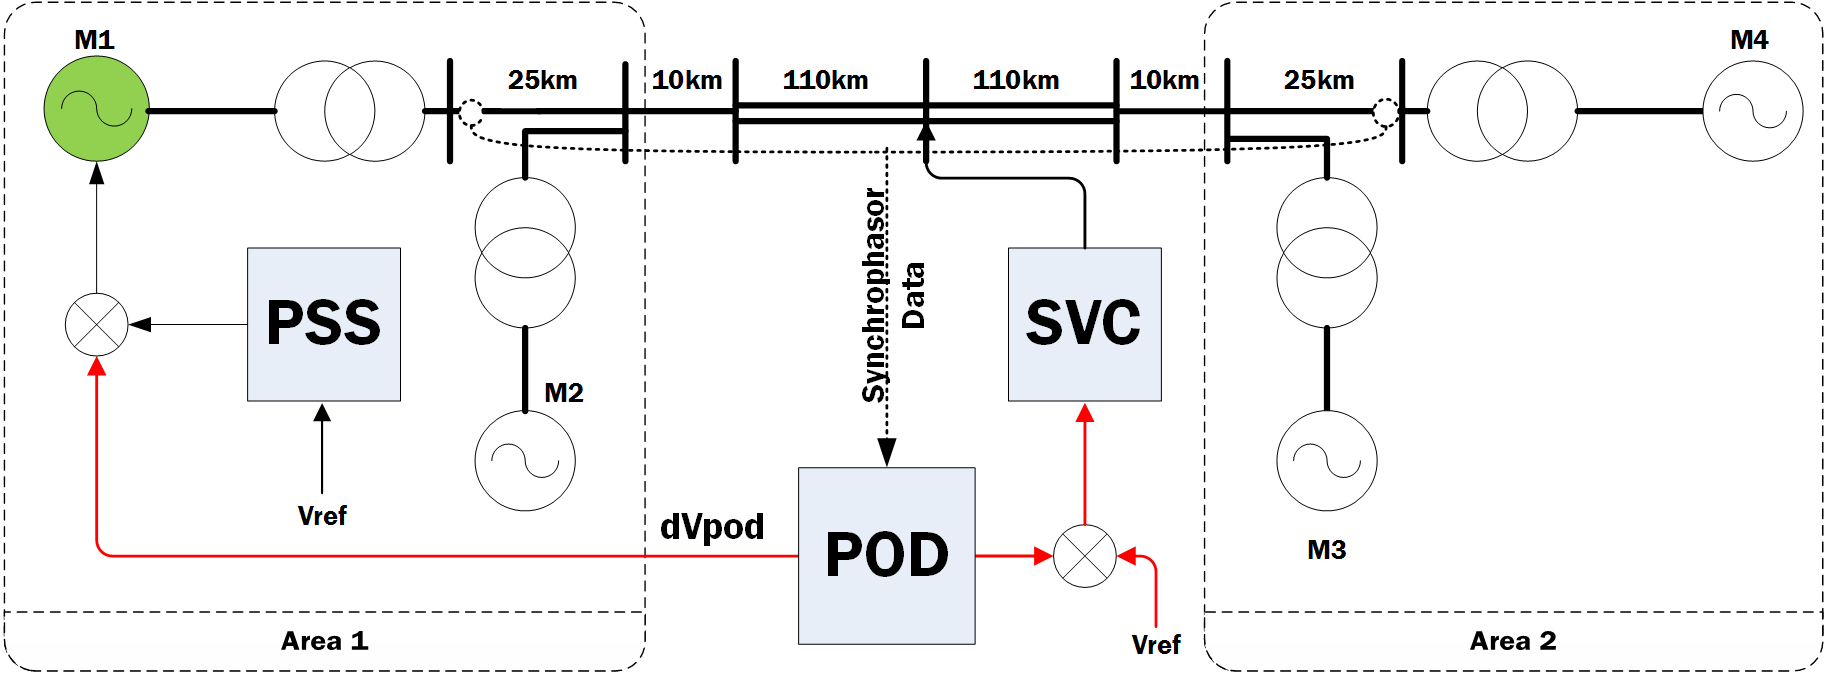
\includegraphics[width=3.5in]{Kundur2Area_outline_multi.png}
\caption{Modified Two-Area Four-Machine network}
\label{NetworkOutline}
\end{figure}

The two-area network \cite{KundurTwoArea} is known to be unstable without external damping control. The difference between the rotational inertias of two of the machines, in an otherwise symmetric network gives rise to the 0.64Hz inter-area mode. The \textsc{Simulink} model used here implements damping control using a supplementary signal generated from a PSS and applied to the excitation system of each of the machines to achieve steady-state stability and also to damp out the inter-area mode. This model was modified to have a damping control system only at Machine M1 in Area-1 (see~Figure~\ref{NetworkOutline}). All other machines have their PSS's disconnected. This configuration was  verified to be able to both achieve stability and to be able to restore the system to stability after the application (and subsequent clearing) of an 8 cycle, three-phase to ground fault. The original model uses a PSS tuned to achieve maximum damping, given the operating conditions. To demonstrate a potential application scenario for the developed POD prototype, the performance of the PSS is degraded so that it is still able to provide damping but takes substantially longer (Figure \ref{PSS_Degrade}). This figure shows the system response to a 200ms perturbation in the voltage reference of machine M1. Note that under the action of the sole PSS at machine M1, the inter-area mode is damped and the system is restored to stability. This mimics a real-world situation where an already installed PSS whose performance has degraded over time due to changing network conditions or poor tuning.\\

Details of the two-area model parameters are listed in Appendix \ref{LiiteC}.\\


\subsection{Two-Area Model Preparation - FACTS Device}

The second application in Figure \ref{NetworkOutline} is to use the WAPOD output as a modulating input to an SVC's excitation system. The two-area model was prepared for simulation in the same way as in the previous case except that the PSS at each machine was included. The SVC model used was an average valued model, identical to that used in \cite{PhasorPODImplement}. The SVC was connected at the mid-point of the two area network. As proved by Chow and Larsen in \cite{sVARdamp}, this is the point where voltage swings will be the greatest and also where the SVC can be most effective at damping power swings As before, two parallel and identical implementations of the Phasor-POD algorithm were used, one implemented in SIMULINK and the other on the cRIO. Either could be switched in at a given time. It is important to note here that when the hardware-POD algorithm was switched in, the PSS's at each of the four machines were disconnected, leaving the SVC as the sole control and damping device in the network. The ability of the SVC to keep the network stable and also to restore it to stability was verified with an off-line simulation using the Phasor-POD implemented in \textsc{Simulink}. Also, the performance of the PSS's were not degraded as the Phasor-POD algorithm would not be running in parallel with them.

\subsection{Real-Time Simulation}
The modified network in each case was grouped into sub-systems and prepared for simulation in RT-LAB. The simulation time step chosen was 50$\mu$s. Outputs and inputs of the real-time simulator would be updated every 50$\mu$s. Current and voltage measurements were taken from the points marked in Figure \ref{NetworkOutline} and were extracted from the analogue outputs of the real-time simulator. The damping signal \emph{dVpod} in Figure~\ref{NetworkOutline} was generated at two points; one in the real-time simulation itself using a Simulink implementation of the Phasor POD algorithm and one externally on the cRIO. Both signals were generated simultaneously and either one could be switched in for use in the simulation.

\section{Testing \& Results}\label{Results}

Testing the operation of the hardware prototype involved using the HIL\footnote{Hardware in the Loop} setup outlined in Figure~\ref{Hardware_Outline} and verifying whether steady state stability could be maintained in the simulated two-area network. Once this was demonstrated, the inter-area mode was excited by changing the voltage reference $V_{ref}$ of Machine M1. The oscillations caused by this disturbance would then be damped out by the PSS in tandem with the Phasor POD algorithm. The POD algorithm implemented in \textsc{Simulink} uses the locally available active power measurements as input. In the case of the Generator PSS, this is the active power measured at the terminals of the generator. In the case of the SVC, the active power at the mid-point of the interconnecting line (also the point of connection of the SVC) is used as an input. The WAPOD prototype is also able to use this same signal as input in each case but can also exploit other data contained in the synchrophasor data stream.

\subsection{SVC Excitation Supplementary Input}
Figure \ref{SVC_Plots} illustrates the response of the hardware controller to a small disturbance at machine M1. This disturbance is a 5\% change for 200ms in the reference voltage of the AVR. This is sufficient to excite the inter-area mode. The best damping performance is achieved using voltage angle difference as a damping input to the Phasor-POD algorithm. This supports the theoretical results predicted by Chompoobutrgool and Vanfretti in \cite{Yuwa}. A frequency analysis of each of these responses shows that the dominant mode in each response is the 0.64Hz inter-area mode. This is evident in Figure \ref{FourierAngle}, which presents the magnitude spectrum of the controller response with voltage angle as input.
\begin{figure}[!th]
\centering
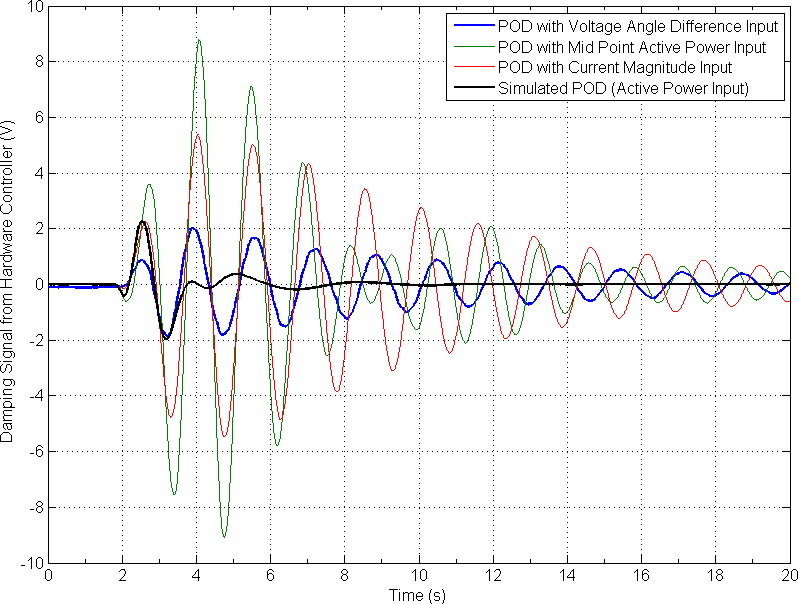
\includegraphics[width=3.5in]{SVC_ResponseComparison_Labelled_NoVMag.png}
\caption{Controller Response Comparison : Supplementary SVC Excitation Input}
\label{SVC_Plots}
\end{figure}

\begin{figure}[!th]
\centering
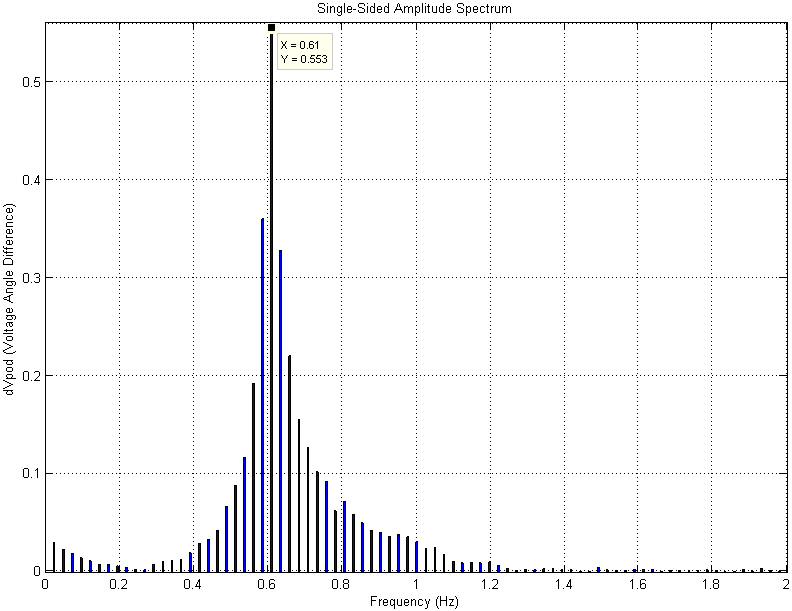
\includegraphics[width=3.5in]{VoltageAngleDiff.png}
\caption{Controller Response Comparison : Supplementary SVC Excitation Input}
\label{FourierAngle}
\end{figure}

All data presented in Figure \ref{SVC_Plots} was captured in the real-time simulator. Data was also recorded at other points such as at the PDC but these have a lower resolution and are not presented here. As further proof of the results presented in this work, the output of the hardware controller is captured directly and presented on an oscilloscope (Figure \ref{ScopeCapture}).

\begin{figure}[!th]
\centering
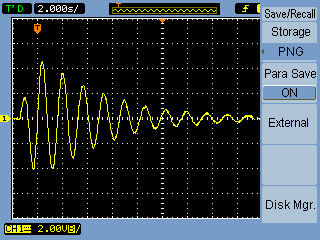
\includegraphics[width=3.5in]{Best_sample.png}
\caption{Controller Response with Voltage Angle Difference input Captured on Oscilloscope}
\label{ScopeCapture}
\end{figure}

\subsection{Generator Excitation Supplementary Input}

The controller response to a small disturbance when operating in tandem with a degraded PSS is shown in Figure~\ref{Generator_Plots}. It is evident that the combination of the WAPOD and the PSS is significantly better than the PSS alone in every case. It can also be noted that the shape of the response shows a significant deviation from that in Figure~\ref{SVC_Plots}, where the dominant 0.64Hz mode is clearly visible. Also evident from Figure~\ref{Generator_Plots} is the fact that the damping performance of the WAPOD changes significantly as its input is changed. Using the voltage angle difference as input provides the best performance. The performance with the simulated POD algorithm is not shown in Figure~\ref{Generator_Plots} for clarity,the performance of the WAPOD with the voltage angle difference input is very close to the performance of the simulated POD algorithm that uses active power as input. This performance is achieved despite the presence of a stochastic time delay and noise in the input measurements of the WAPOD. As in the case with the SVC, the theoretical results in \cite{Yuwa} agree with the experimental results.

\begin{figure}[!th]
\centering
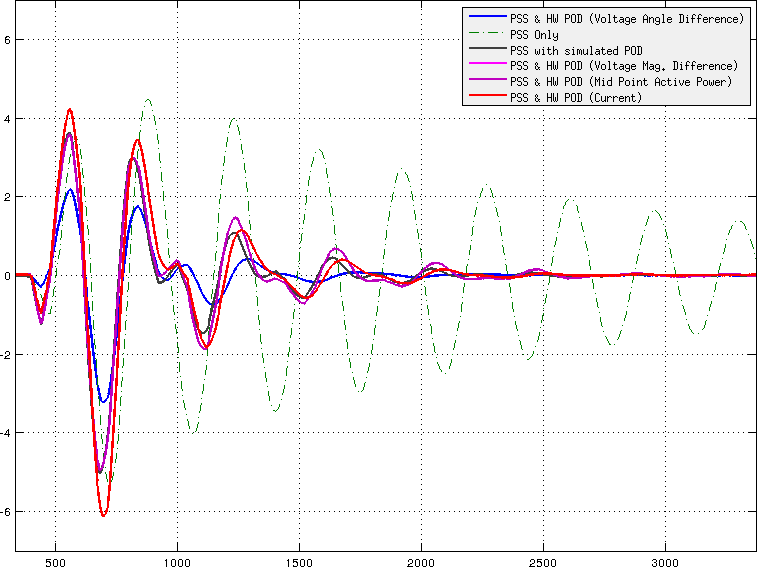
\includegraphics[width=3.5in]{Wide_Area_ResponseComparison_SamePlot.png}
\caption{Controller Response Comparison : Supplementary Generator Excitation Input}
\label{Generator_Plots}
\end{figure}
%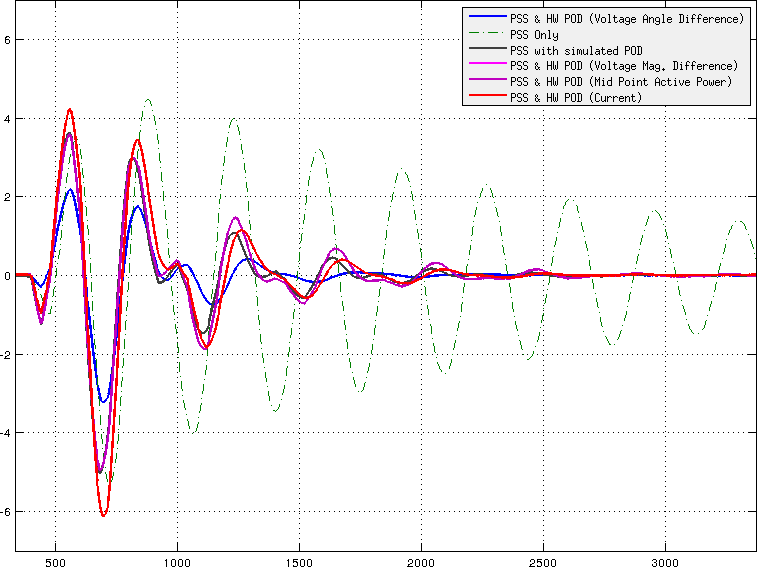
\includegraphics{Wide_Area_ResponseComparison_SamePlot.png} 

%\section{Additional Inputs}

\section{Challenges}\label{Challenges}

\subsection{Time Delays}

The Phasor POD algorithm running in SIMULINK has close to zero time delay between network behaviour changing and the controller responding. The same algorithm, when run on the cRIO, receives data with a stochastic delay. Figure \ref{Hardware_Outline} illustrates the complete data path and from this, it is evident that several sources of time delay exist. Sections such as the analogue amplifiers, the FPGA execution speed (a constant 50$\mu$s), the real-time section of the cRIO and the PDC all represent fixed, non-zero time delays. Sections such as the D/A and A/D conversion in the real-time simulator also add a deterministic time delay. However, sections of the data path such as communication over a TCP/IP network and the PC used to extract raw measurement data from the synchrophasor stream all represent variable delays. These delays all contribute to a delayed response from the cRIO. This delay allows for a network disturbance to grow slightly before the cRIO starts responding. It also has the effect of changing the phase compensation required in the Phasor-POD algorithm. Though the delay cannot be compensated for, the phase compensation needed can be changed depending on the measured delay. Presently, the phase compensation required is determined iteratively though this can be automated using time-stamped data.\\

%In a direct comparison between the simulated Phasor-POD and one running on the cRIO, the time delay will be 

\subsection{Analogue Limits and Noise}
The original POD (Phasor Oscillation Damper) algorithm~\cite{PhasorPOD} was developed and simulated in an ideal, noise-free environment with zero delay. More importantly, no limits are imposed on the magnitude of either the controller's inputs or outputs when it is simulated. In contrast, a hardware-based implementation that uses analogue signals is constrained by the analogue signal magnitude limits.\\

Consider the analogue outputs of OPAL RT's eMEGASIM simulator \cite{OPALemegasim}.

\begin{itemize}
\item \textbf{Analogue Outputs} : Number: 32 (+/-16V and +/-10mA)
\item \textbf{Analogue Inputs} : Number: 128 (+/-100V and +/-10mA)
\end{itemize}

These are low level outputs and can be directly connected to the PMU inputs. However, the inputs modules of typical PMU's are rated for 0-300V and a 0-16V analogue signal will not use a significant portion of this range. Additionally, a signal of such a small magnitude will be contaminated by noise and will consequently have a poor Signal to Noise ratio. A similar argument can be made for the current outputs.\\

The output of the simulated POD can vary over several orders of magnitude, ranging from $10^{5}$ at times of peak damping to as small as $10^{-3}$ once the oscillation magnitude  becomes small. It is difficult to accurately recreate analogue signals with such vast dynamic ranges. The voltage output module used with the cRIO here had a 24-bit resolution and was limited to 10V in magnitude. Any values generated by the POD algorithm that were greater in magnitude that 10V would cause output saturation. All these issues meant that signal magnitudes had to be amplified in certain cases to use the full measurement ranges or had to be limited in other cases, so as to capture variations without saturation.\\

\subsection{Loop Rates and FPGA Resources}\label{looprate}
The most significant challenge in the real-time implementation of the Phasor-POD algorithm was the fact that different sections of the hardware control loop run at different loop rates or step sizes. Added to this was the fact that the real-time simulator generated data every 50$\mu$s and thus expected data from the HIL setup at the same rate while the rest of the HIL setup did not support such a high data rate. The PMU\rq{s} used supported a maximum data reporting rate of 50 samples/second. Table~\ref{ex:LoopRates} lists the different components of the HIL setup together with their respective loop rates.
\begin{table}[!ht]
\caption{Comparison of Loop Rates of Different Components}\label{ex:LoopRates}
\begin{center}
\begin{tabular}{|l|c|c|}
\hline \textbf{Element} & \textbf{Loop Rate} & \textbf{Mode} \\
\hline OPAL RT Simulator & 50$\mu$s & Real Time \\ 
\hline PMU (cRIO) & 20msec & Real Time \\ 
\hline Workstation Computer& 20msec & Not Real Time \\ 
\hline POD - RT Section & 20msec & Real Time \\ 
\hline POD - FPGA & 50$\mu$s & Real Time \\ 
\hline 
\end{tabular}
\end{center}
\end{table} 

50$\mu$s was chosen for the FPGA loop rate in order to match the loop rate of the real-time simulator. This was to ensure that data was always available at the analogue input of the simulator and no erroneous data points were read. The 50$\mu$s loop rate of the FPGA meant that new data was expected every 50$\mu$s, corresponding to a 2000s/s sampling rate. The fastest execution speed of the real-time section of the cRIO was 1ms, significantly slower than the FPGA\rq{s} speed. New synchrophasor data was available from the PMU\rq{s} only every 20ms. One solution to this problem was to upsample the synchrophasor data, interpolate between consecutive data points and then stream this data to the Phasor-POD algorithm on the FPGA. A FIFO\footnote{First In First Out} buffer would be used to buffer the data generated by the up-sampling process as it was gradually consumed by the FPGA. The major problem with this method was that the up-sampling process on the RT controller is computationally intensive and would not run at the required 20ms loop rate.\\

An alternative solution would be to implement a sample and hold algorithm on the FPGA. As data was extracted every 20ms, the RT controller would receive this data and send it to the FPGA. This value would then be held constant till the next data point arrives. This was implemented and found to work satisfactorily. In essence, the only difference between the Phasor-POD algorithm running the SIMULINK simulation and that on the cRIO was the data rates of their input data. The simulated POD received new data every 50$\mu$s while the cRIO-based POD received data every 20ms.

%A significant problem here was the fact that the synchrophasor data-extraction software running the on the workstation computer was not running in real-time. This, together with the TCP/IP sections, introduced stochastic delay in the control loop. 

\section{Further Work}\label{Future}

The WAPOD prototype as developed in this work demonstrates the possibilities of using wide area synchrophasor data for damping control. The prototype here is, however, dependent on manual input for signal selection and algorithm parameter values. These two processes can be automated by having the WAPOD itself monitor the various input signals and intelligently select the one having the highest observability of a particular mode. The algorithm parameters can also be determined adaptively on the WAPOD itsef. On the same lines, this can further be extended to include selection among several measurement locations on the network. The fact that a stochastic time delay is introduced by unwrapping the synchrophasor data stream on a desktop computer can be addressed by performing this function on the WAPOD controller (here, the cRIO) itself.

\section{Conclusion}\label{Conclusion}
This work has demonstrated the feasibility of using wide-area power system data in the design of an oscillation damping controller. The generic nature of the developed controller was demonstrated by using an identical implementation with mere changes in paramaters to suit the controlled device's input requirements and capabilities. The performance of the WAPOD can be improved by exploiting the full range of data available in a synchrophasor data stream.The flexibility of synchrophasor data was demonstrated and the wide range of inputs possible from this were also tested. The results from this work serve as a proof-of-concept to what?





% if have a single appendix:
%\appendix[Proof of the Zonklar Equations]
% or
%\appendix  % for no appendix heading
% do not use \section anymore after \appendix, only \section*
% is possibly needed

% use appendices with more than one appendix
% then use \section to start each appendix
% you must declare a \section before using any
% \subsection or using \label (\appendices by itself
% starts a section numbered zero.)
%


\appendices
%\section{Proof of the First Zonklar Equation}
\section{Two Area Four-Machine Model Parameters\label{LiiteC}}

Two-area model parameters (Similar to those used in \cite{KundurTwoArea})\\
%\renewcommand{\theequation}{C\arabic{equation}}
%\setcounter{equation}{0}  
%\renewcommand{\thefigure}{C\arabic{figure}}
%\setcounter{figure}{0}
%\renewcommand{\thetable}{C\arabic{table}}
%\setcounter{table}{0}

\begin{table}[!ht]
\caption{Common Generator Parameters used in Simulink Two Area Model}
\begin{center}
%\bigskip
\begin{tabular}{|c|c|c|c|c|c|}

\hline $ X_{d} $ & 1.8  &$ {X}_{d}^{\prime } $  & 1.8  & $ {X}_{d}^{\prime \prime } $ & 0.25  \\ 
\hline $ X_{q} $ & 1.7  &$ {X}_{q}^{\prime } $  & 0.55 & $ {X}_{q}^{\prime \prime } $ & 0.25 \\ 
\hline $ X_{l} $ & 0.2  & $ R_{a} $ & 0.0025  & $ K_{d} $  & 0 \\ 
\hline $ {T}_{d0}^{\prime } $ &8s  & $ {T}_{q0}^{\prime } $ & 0.4s & - & - \\ 
\hline $ {T}_{d}^{\prime \prime } $ & 0.03s & $ {T}_{q}^{\prime \prime } $ & 0.05s  &- &-  \\ 
\hline $ A_{SAT} $& 0.015 & $ B_{SAT} $ & 9.6 & $ \psi_{T1} $  & 0.9 \\ 
\hline 
\end{tabular}
\end{center}
\end{table}
\emph{N.B. All Parameters in p.u., on Generator Base}\\

Step Up Transformer Impedance : $0+j0.15$\\

\begin{table}[!ht]
\caption{Transmission line parameters}
\begin{center}
\begin{tabular}{|c|c|}
\hline $r=0.0001$ pu/km & $x_{l}=0.001$ pu/km \\
\hline $b_{c}=0.00175$ pu/km &  Nominal Voltage : 230kV\\ 
\hline 
\end{tabular}
\end{center}
\end{table}

\begin{table}[!ht]
\caption{Self-excited DC exciter Parameters (common to all generators)}
\begin{center}
\begin{tabular}{|c|c|c|c|}
\hline  $ K_{A} = 20 $& $ T_{A} = 0.055 $ & $ T_{E} = 0.36 $ & $ K_{F} = 0.125 $ \\ 
\hline $ T_{F} = 1.8 $ & $ A_{ex} = 0.0053 $ & $ B_{ex} = 1.075 $ & $ T_{R} = 0.05 $ \\ 
\hline 
\end{tabular} 
\end{center}
\end{table}
% you can choose not to have a title for an appendix
% if you want by leaving the argument blank
\section{Modifications Made to PSS Model}

The default simulation model supplied with the \texttt{power\_PSS} example in \textsc{Matlab} has three types of PSS models \cite{MATLABexample} : an MB-PSS, a $\Delta\omega $-PSS and a $\Delta P_{a}$ PSS. The comparison of the three as presented in \cite{MATLABexample} concludes that the performance of the MB-PSS is the best. This model is thus, not used when modulating the PSS output with the Phasor-POD algorithm. Instead, the $\delta P_{a}$ PSS is used. The PSS model here is the generic PSS model available with SimPowerSystems \cite{PSSDocumentation}.\\

The input to the $\Delta\omega $-PSS is the rotor speed deviation $\Delta\omega $. For an accurate comparison, this was changed to the measured active power measured at the generator terminals, $P_{a}$. The lead-lag block parameters were also changed from $\frac{1 + 50x10^{-3}s}{1 + 1s}$ to $\frac{1 + 50x10^{-3}s}{1 + 6s}$. Parameters here were determined iteratively. The change to the lead-lag block produces the effect in Figure \ref{PSS_Degrade} where the PSS is still able to restore the system to stability but takes almost a minute to damp out the oscillations versus approximately three seconds in the ideal case.\\

%Photos should span two columns or full page.

\section{SmarTS Lab Outline \& Setup Images}

The SmarTS Lab at KTH was set up with the aim of developing wide area monitoring, protection and control (WAMPAC) schemes for the power grid. Much of the infrastructure and activities involve PMU data and the associated communication and computer systems  \cite{SmarTSLab}. The lab is equipped with facilities for real-time (RT) simulations and also RT Hardware-in-the-loop (HIL) tests. A reduced schematic is shown in Figure \ref{fig:SmarTSlabOutline}\\

The core of the setup is the eMEGASIM Real-time simulator from OPAL RT ~\cite{eMEGASIM}. Two \textquoteleft targets' are available,  each running a 12-core 3.3Ghz Intel i7 processor \cite{SmarTSLab}. This allows the running of models created in \textsc{Matlab}/Simulink in real-time. These simulations can interact with external devices through the simulator's low-power analogue outputs and inputs or with data streamed over TCP/IP, UDP etc \cite{SmarTSLab}. In this thesis, the power system under test is simulated on this platform.\\

The analogue outputs and their ratings are listed below:\label{OPALlimits}

\begin{itemize}
\item \textbf{Analogue Outputs} : 32 (+/-16V and +/-10mA)
\item \textbf{Analogue Inputs} : 128 (+/-100V and +/-10mA)
\end{itemize}

The full listing of the simulator's capabilities and interfaces is covered in \cite{SmarTSLab}. Only necessary and relevant details are covered here.\\

The WAMPAC platform includes a Phasor Data Concentrator (PDC) and its associated software from Schweitzer Engineering Laboratories (SEL). Other devices are interfaced with the PDC such as protection relays with embedded PMU functionality, line differential protection relays (ABB), Compact RIO micro-controllers (National Instruments) and analogue signal amplifiers (Megger)\cite{SmarTSLab}. The hardware list here is incomplete and other devices are also used such as a GPS receiver, a relay current and voltage injection kit etc.\\

\begin{figure*}[!t]\label{SetupImage}
\centering
\includegraphics[width=1\linewidth]{./LabView_Numbered}
\caption{Outline of the SmarTS Lab. Corresponding to Numbers: 1: Real Time Simulator, 2: PDC Interface, 3: cRIO Tray, 4: Oscilloscope, 5: Analogue Signal Amplifiers, 6: SEL Protection Relays}
\label{fig:LabView_Numbered}
\end{figure*}

\begin{figure*}[!t]
\centering
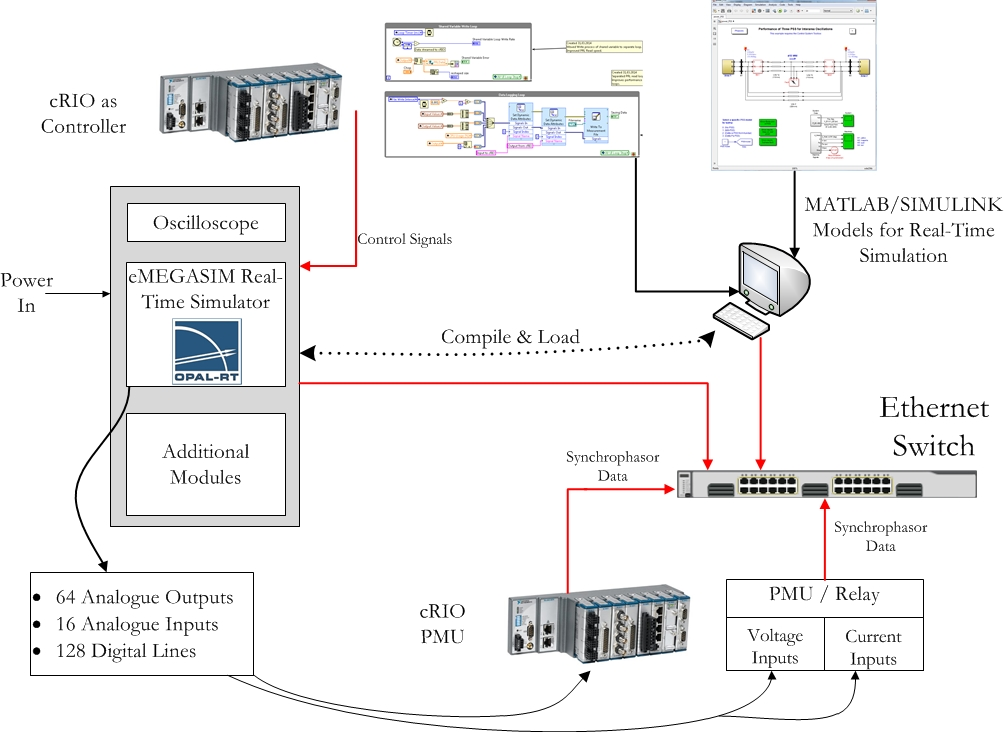
\includegraphics[width=1\linewidth]{./SmarTSlabOutline}
\caption{Outline of SmarTS Lab at KTH}
\label{fig:SmarTSlabOutline}
\end{figure*}

%Appendix two text goes here.


% use section* for acknowledgement
\section*{Acknowledgment}


The authors would like to thank...


% Can use something like this to put references on a page
% by themselves when using endfloat and the captionsoff option.
\ifCLASSOPTIONcaptionsoff
  \newpage
\fi



% trigger a \newpage just before the given reference
% number - used to balance the columns on the last page
% adjust value as needed - may need to be readjusted if
% the document is modified later
%\IEEEtriggeratref{8}
% The "triggered" command can be changed if desired:
%\IEEEtriggercmd{\enlargethispage{-5in}}

% references section

% can use a bibliography generated by BibTeX as a .bbl file
% BibTeX documentation can be easily obtained at:
% http://www.ctan.org/tex-archive/biblio/bibtex/contrib/doc/
% The IEEEtran BibTeX style support page is at:
% http://www.michaelshell.org/tex/ieeetran/bibtex/
%\bibliographystyle{IEEEtran}
% argument is your BibTeX string definitions and bibliography database(s)
%\bibliography{IEEEabrv,../bib/paper}
%
% <OR> manually copy in the resultant .bbl file
% set second argument of \begin to the number of references
% (used to reserve space for the reference number labels box)
\begin{thebibliography}{1}

\bibitem{PhasorPOD} 
L.~\"{A}ngquist and C.~Gama  \emph{Damping Algorithm based on Phasor Estimation} in Power Engineering Society Winter Meeting, 2001. IEEE, Volume 3, pp. 1160 - 1165  

\bibitem{KundurTwoArea} 
M.~Klein, J. G.~Rogers and P.~Kundur \emph{A fundamental study of inter-area oscillations in Power Systems} IEEE Trans, PWRS, no. 6, pp. 914-921, 1991. 

\bibitem{eMEGASIM} \emph{eMEGASIM Power Grid Real-Time Digital HArdware in the Loop Simulator} Available Online at : \url{http://www.opal-rt.com/}

\bibitem{Dmello} F. P.~Dmello, and. \ C.~Concordia
  \emph{Concepts of Synchronous Machine Stability as Affected by Excitation Control} IEEE TRANSACTIONS ON POWER APPARATUS AND SYSTEMS, vol. PAS 88, no. 4, 1969. 
  
\bibitem{localREMcomparison}  M. E.~Aboul-Ela, A. A.~Sallam, J. D.~McCalley and A. A.~Fouad, \emph{Damping Controller Design for Power System Oscillations Using Global Signals}, IEEE trans. on Power Systems, Vol. 11, No. 2, May 1996, pp. 767-773
  
\bibitem{PhasorPODImplement} M.~Shoaib Almas and L.~Vanfretti, \emph{Implementation of Conventional PSS and Phasor Based POD for Power Stabilizing Controls for Real-Time Simulation}, IEEE IES IECON14, 29 Oct-1 Nov, 2014, Dallas, USA.

\bibitem{OPALemegasim} eMEGAsim PowerGrid Real-Time Digital Hardware in the Loop Simulator — Opal RT, [Online]. Available: \url{http://www.opal-rt.com/}

\bibitem{Chaudhuri} N.S.~Chaudhuri, R.~Majumder and B~ Chaudhuri \emph{Interaction between conventional and adaptive phasor power oscillation damping controllers} in Power and Energy Society General Meeting, 2010 IEEE Minneapolis, MN, 2012 pp. 1-7

\bibitem{SmarTSLab} L.~Vanfretti.; M.~Chenine; M.S.~Almas; R.~Leelaruji; L.~Angquist; L.~Nordstrom, "\emph{SmarTS Lab — A laboratory for developing applications for WAMPAC Systems}," Power and Energy Society General Meeting, 2012 IEEE , vol., no., pp.1,8, 22-26 July 2012

\bibitem{sVARdamp} E.V~Larsen and E.H~Chow, General Electric Company, NY, \emph{Application of Static VAR Systems for System Dynamic Performance}, 1987 IEEE pp. 43-46

\bibitem{Yuwa}  L.~Vanfretti, Y.~Chompoobutrgool, and J.H.~Chow, \emph{Chapter 10: Inter-Area Mode Analysis for Large Power Systems using Synchrophasor Data}, Book Chapter, in Coherency and Model Reduction of Large Power Systems, Joe H. Chow (Ed.), Springer, 2013. Available Online at \url{http://www.springer.com/energy/systems%2C+storage+and+harvesting/book/978-1-4614-1802-3}

\bibitem{cRIO9081} \emph{Operating Instructions and Specifications Compact RIO NI cRIO-9081/9082}, National Instruments, Available Online at \url{http://www.ni.com/pdf/manuals/375714a.pdf}
  
\bibitem{cRIO9076} \emph{Operating Instructions and Specifications Compact RIO NI cRIO-9075/9076}, National Instruments, Available Online at \url{http://www.ni.com/pdf/manuals/375650b.pdf}

\bibitem{LabviewTemplate} \emph{FPGA Control on Compact RIO Sample Project Documentation}, National Instruments, Available Online at \url{http://www.ni.com/white-paper/14137/en/}

\bibitem{SDK} Vanfretti, Luigi and Aarstrand, Vemund H. and Almas, M. Shoaib and Peri\'c, Vedran S. and Gjerde, Jan O. , \emph{A Software Development Toolkit for Real-Time Synchrophasor Applications},  IEEE PES Grenoble PowerTech, 2013

\bibitem{Chaudhuri} N.S~Chaudhuri, R~Majumder and B~Chaudhuri , \emph{Interaction between conventional and adaptive phasor power oscillation damping controllers} in Power and Energy Society General Meeting, 2010 IEEE Minneapolis, MN, 2012 pp. 1-7

\bibitem{MATLABexample} I~Kamwa \emph{Performance of Three PSS for Interarea Oscillations} SimPowerSystems Examples, \textsc{Matlab} R2011a

\bibitem{PSSDocumentation} \emph{Generic Power System Stabilizer} Documentation distributed with \textsc{Matlab} R2014a Available online at \url{http://www.mathworks.se/help/physmod/sps/powersys/ref/genericpowersystemstabilizer.html}

\end{thebibliography}

% biography section
% 
% If you have an EPS/PDF photo (graphicx package needed) extra braces are
% needed around the contents of the optional argument to biography to prevent
% the LaTeX parser from getting confused when it sees the complicated
% \includegraphics command within an optional argument. (You could create
% your own custom macro containing the \includegraphics command to make things
% simpler here.)
%\begin{biography}[{\includegraphics[width=1in,height=1.25in,clip,keepaspectratio]{mshell}}]{Michael Shell}
% or if you just want to reserve a space for a photo:

\begin{IEEEbiography}[{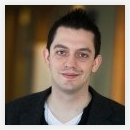
\includegraphics[width=1in,height=1.25in,clip,keepaspectratio]{lvanfretti.PNG}}]{Luigi Vanfretti}
Biography text here.
\end{IEEEbiography}

\begin{IEEEbiography}[{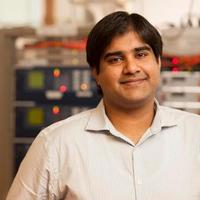
\includegraphics[width=1in,height=1.25in,clip,keepaspectratio]{msalmas.PNG}}]{M S Almas}
Biography text here.
\end{IEEEbiography}

% if you will not have a photo at all:
\begin{IEEEbiographynophoto}{Eldrich Rebello}
Biography text here.
\end{IEEEbiographynophoto}

% insert where needed to balance the two columns on the last page with
% biographies
%\newpage

% You can push biographies down or up by placing
% a \vfill before or after them. The appropriate
% use of \vfill depends on what kind of text is
% on the last page and whether or not the columns
% are being equalized.

%\vfill

% Can be used to pull up biographies so that the bottom of the last one
% is flush with the other column.
%\enlargethispage{-5in}



% that's all folks
\end{document}


